\chapter{Implementacja}
W poniższym rozdziale opisane zostały prace nad modułem, przyczyny oraz uzasadnienie poszczególnych decyzji projektowych oraz problemów, które po drodze wyniknęły. Finalna architektura wraz z pełnym wyjaśnieniem funkcjonalności poszczególnych komponentów została opisana w rozdziale \ref{chapter_System_Architecture}.

\section{Podstawowy projekt zapoznawczy}
Pierwszym krokiem w utworzeniu modułu było utworzenie aplikacji testowej. Używa ona tych samych bibliotek oraz API co końcowy moduł, ale w formie okrojonej, nie realizując założeń architektury systemu, a jedynie MVP - Minimal Viable Product. Takie rozwiązanie pozwala na zapoznanie się z praktycznym wykorzystaniem używanych później interfejsów, a także na stworzenie wzorca do pierwszej implementacji faktycznego modułu docelowego.

Prace nad aplikacją rozpoczęto od utworzenia rozwiązania w programie Visual Studio 2022 na podstawie załączonego do niego wzorca - \textit{Direct3D 11 Game Win32} \cite{GitHub:walbourn:directx-vs-templates}, zawierającego prekonfigurowany projekt wykorzystujący Direct3D oraz DirectXTK. W ramach szablonu zawarte są też podstawowe metody tworzenia zasobów używanych w ramach D3D, a także przyjęta przez jej autora struktura sterowania przepływu kodu - inna od zaplanowanej w ramach modułu. Następnie dodane zostały zgodne z założeniami biblioteki i przetestowano poprawność konfiguracji. Do tak skonfigurowanego projektu dodane zostały metody wczytywania geometrii podstawowych modeli za pomocą biblioteki assimp, a także bez określonej struktury kod odpowiedzialny za ich dodatkową obróbkę oraz finalne renderowanie. Projekt aplikacji zapoznawczej został zakończony implementacją widoku z obracającym się, kolorowym trójkątem, przedstawionym na rys. \ref{Impl_TemplateProject}.

\begin{figure}[h!]
	\centering
	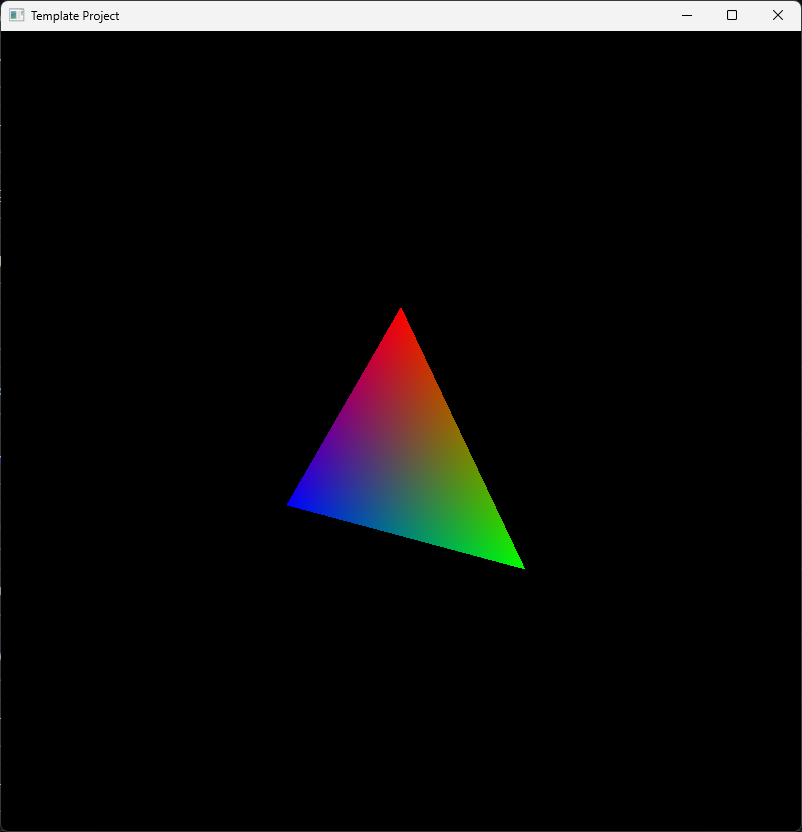
\includegraphics[width=300px]{images/impl/1_template_project.png}
	\caption{Statyczny obraz obracającego się trójkąta w ramach projektu zapoznawczego.}
	\label{Impl_TemplateProject}
\end{figure}

\vfill
\clearpage

\section{Moduł rdzeniowy}
Tak przygotowany projekt umożliwiał względnie proste utworzenie aplikacji renderującej wczytany z dysku model, ale ze względu na brak konkretnej architektury oraz celu nie nadawał się do dalszego rozwoju. Kolejnym krokiem było więc przeniesienie już istniejących funkcjonalności do formy zgodnej z docelową architekturą, możliwą do dalszego rozwoju. W tym celu utworzona została podstawowa struktura \textbf{D3DEngine} (przemianowana później na \textbf{D3DCore}), przechowująca referencje do rdzeniowych zasobów systemu Direct3D oraz okna, a także odpowiedzialna za tworzenie, odpowiednie zarządzanie, użyczanie i zwalnianie tych zasobów. W kolejnym kroku do klasy dodane zostały nadpisywalne obiekty wskaźników na funkcje zdarzeń, wywoływanych przy niektórych interakcjach użytkownika z oknem - takich jak jego przesunięcie, zmiana rozmiaru czy aktywnego okna. Poprawiona została także wydajność ze względu na przejście ze starego trybu publikacji klatek obrazu - DXGI\_SWAP\_EFFECT\_BLIT - na nowy - DXGI\_SWAP\_EFFECT\_FLIP. 

\subsection{Wiele okien - wiele problemów}
W tym momencie zapadła decyzja, według której powinna być możliwość niezależnego działania wielu instancji modułu jednocześnie, co pozwoliłoby na utworzenie aplikacji klienta z funkcjonalnością otwierania wielu okien w ramach jednej aplikacji. Z takim podejściem wiąże się natomiast problem - WinAPI posiada możliwość zdefiniowania funkcji odpowiadającej na event zdarzeń okna \textit{(WndProc)}, ale bez bezpośredniej możliwości powiązania uchwytu okna do własnej struktury go reprezentującej. Po wielu testach różnych rozwiązań ostatecznie problem został rozwiązany pewnym obejściem. Przy tworzeniu okna wskaźnik na strukturę \textit{Window} zostaje przekazany jako ostatni argument funkcji CreateWindowEx - \textit{(lpParam)}. Następnie między WinAPI, a faktycznym eventem WndProc dodany zostaje pośrednik - WndProcDispatcher. Nasłuchuje on konkretnych typów zdarzeń i jeśli otrzyma event typu \textit{WM\_NCCREATE}, oznaczający utworzenie nowego okna, pobiera wskaźnik do struktury \textit{Window} przekazany jako pole struktury \textit{LPCREATESTRUCT} w argumencie lParam. Następnie wykonuje powiązanie z uchwytem do okna przy pomocy mechanizmu \textit{SetWindowLongPtr()}. Dzięki takiemu podejściu w kolejnych wywołaniach \textit{WndProcDispatcher} możliwe jest pobranie wskaźnika do powiązanej z uchwytem struktury przy pomocy funkcji \textit{GetWindowLongPtr()}, a w związku z tym wywołanie metody \textit{WndProc} na odpowiednim oknie. Pseudokod realizujący opisany mechanizm został przedstawiony na listingu \ref{lst:module:WndProcDispatcher}.

\vfill

\begin{lstlisting}[caption={Pseudokod integracji wskaźnika okna z uchwytem HWND}, label={lst:module:WndProcDispatcher}]
void Window::Create() {
 ...
 CreateWindowEx(..., this);
 ...
}

LRESULT WndProcDispatcher(HWND hwnd, UINT message, (...), LPARAM lParam) {
 if (message == WM_NCCREATE) {
     Window* win = (LPCREATESTRUCT)lParam -> lpCreateParams;
     SetWindowLongPtr(hwnd, GWLP_USERDATA, win);
 }
	
 Window* win = GetWindowLongPtr(hwnd, GWLP_USERDATA);
 return win->WndProc(...);
}
\end{lstlisting}

\subsection{Mesh i typy wierzchołków}
Kolejnym napotkanym problemem okazał się być temat typu wierzchołków w ramach modeli i mesh'y. Do poprawnego działania Direct3D wymaga określenia struktury danych wejściowych w ramach mechanizmu InputLayout, która zmienia się w zależności od użytej struktury opisującej typ wierzchołków. Oczywistym rozwiązaniem byłoby użycie mechanizmu szablonowania z języka C++, ale wymagałoby to ręcznego i zewnętrznego definiowania implementacji metody zwracającej D3DInputLayout dla każdego typu wierzchołka z osobna, co jest bardzo podatnym na błędy i nieprzejrzystym rozwiązaniem. Tutaj także udało się znaleźć lepsze rozwiązanie, którym okazał się być wprowadzony w ramach C++20 mechanizm \textit{concepts} \cite{cpp20:concepts:2025}. W ramach tego mechanizmu możliwe jest zdefiniowanie \textit{konceptu}, czyli ograniczeń dla typów szablonowych narzucających im konieczność zawarcia określonej metody. Dzięki temu utworzony został koncept \textit{VertexTypeConcept}, który wymaga utworzenia metody \textit{GetInputLayout()}, zwracającej D3DInputLayout przystosowany do pracy z danym typem.

\subsection{Lewoskrętny układ współrzędnych}
Przewijającym się przez cały proces developmentu - a w tym momencie po raz pierwszy - problemem był także przyjęty jako zalecany w ramach Direct3D lewoskrętny układ współrzędnych, w którym oś +Z rośne wraz z głębokością "w ekranie". Jest to przeciwieństwo układu prawoskrętnego z odwróconą osią Z, wykorzystywanego przez większość konkurencyjnych API, takich jak OpenGL i Vulkan. Duża część otwarto-źródłowych bibliotek oraz dostępnej dokumentacji opiera się na drugiej opcji, co skutkowało okazjonalnymi problemami z mieszaniem skrętności układów współrzędnych. Assimp posiada flagę postprocessingu, mającą na celu zmianę układu na lewoskrętny - \textit{aiProcess\_ConvertToLeftHanded} - która wydawała się pomóc na tym etapie, ale ostatecznie nie naprawiła problemu całkowicie, przez co będzie on wracać i zostanie ostatecznie naprawiony dopiero pod koniec pracy nad modułem.

\begin{figure}[h!]
	\centering
	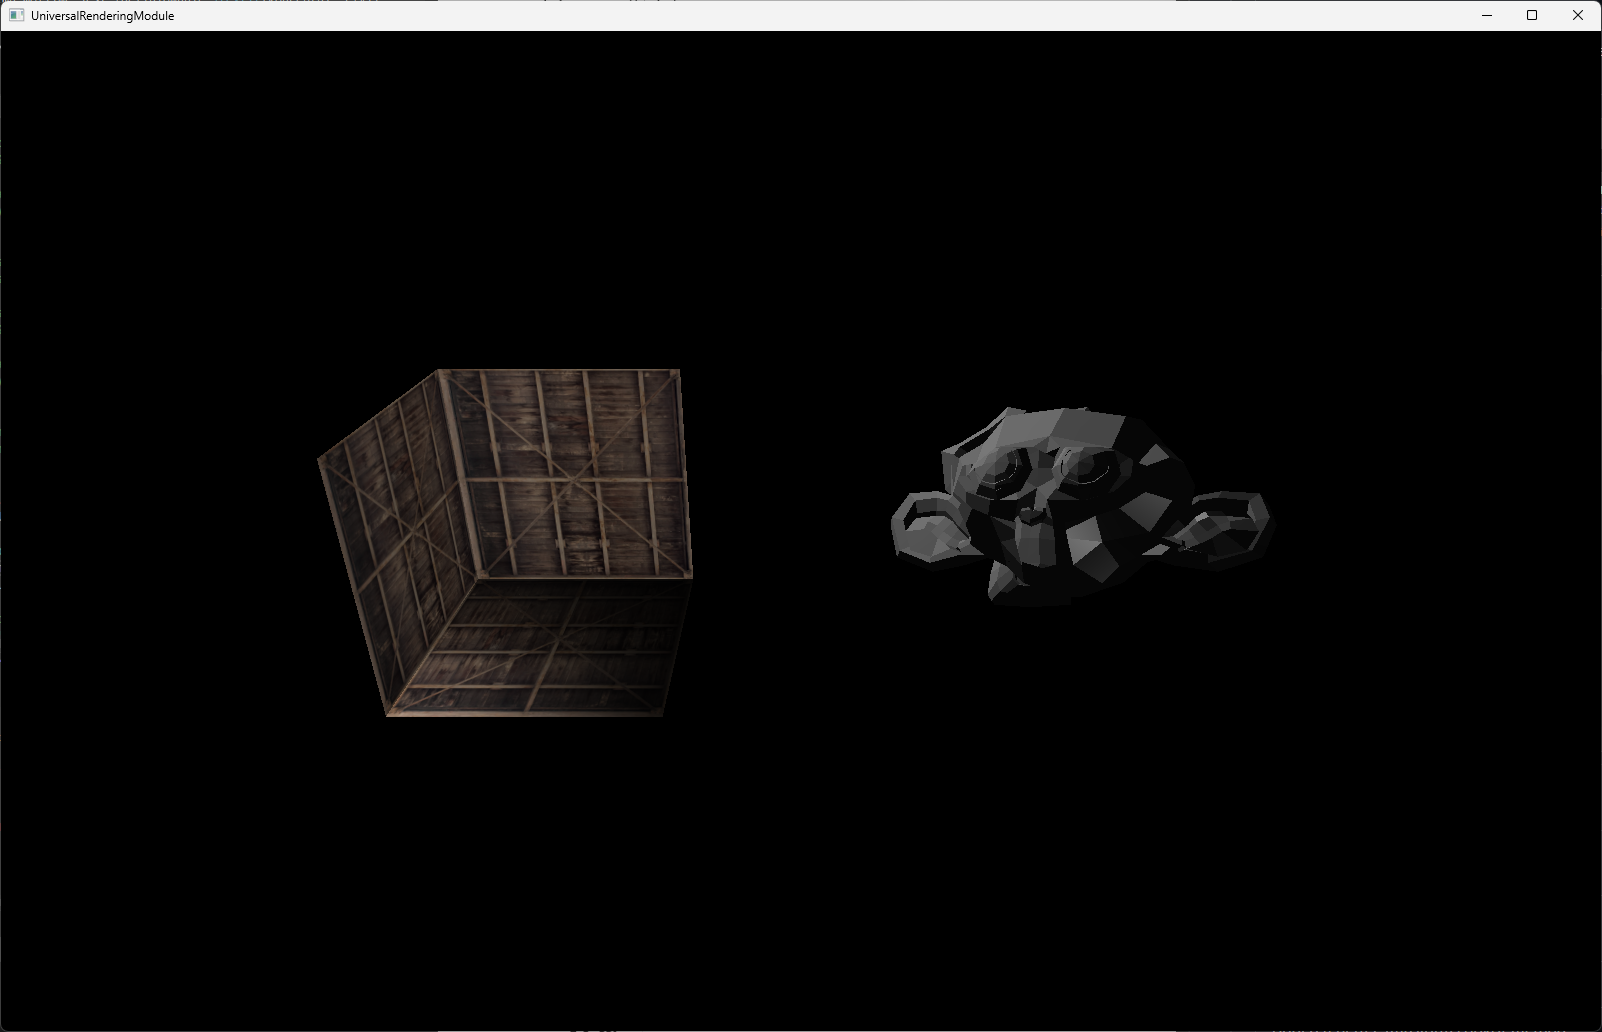
\includegraphics[width=300px]{images/impl/3_inverted_handiness.png}
	\caption{Odwrócona skrętność sortowania wielokątów z widocznym rezultatem w postaci zniekształconych modeli.}
	\label{Impl_InvertedHandiness}
\end{figure}


\subsection{Właściwości materiałów - wczytywanie}
Dane właściwości materiałów, takie jak jego kolor, chropowatość i inne parametry są odczytywane i dekodowane przez assimp przy wczytywaniu plików modeli. Dane te zapisane są jednak w formie tablicy bajtów, niezależnie od tego jaki typ reprezentują. Wczytanie takich danych wiąże się z dwoma potencjalnymi trudnościami - endianness architektury oraz brak wsparcia dla operacji na bitach przy typach zmiennoprzecinkowych.

Pierwszy problem opisuje potencjalną niekompatybilność bitowego zapisu wielobajtowych danych dla różnych architektur. W przypadku systemów Big Endian, dane przechowywane są bajtami w kolejności od najbardziej do najmniej znaczącego, gdzie Little Endian sortuje je odwrotnie. Brak konwersji między typami spowodowałby niepoprawną interpretację danych, a w rezultacie błędne parametry wynikowe. Najważniejsze architektury na rynku są jednak zgodne - procesory ARM oraz x86 operują na założeniu Little Endian \cite{ARM:Developer:Endianness} \cite{Oracle:HelpCenter:x86ByteOrdering}. W związku z tym podjęta została decyzja, aby nie dodawać osobnej ścieżki kodu dla architektur Big Endian, ze względu na niską popularność takich systemów.

Druga trudność wynika ze standardu IEEE 754, opisującego standard typów zmiennoprzecinkowych \textit{(ang. floating point)}, na podstawie którego zaimplementowany został typ float w języku C++. Standard ten zabrania bezpośredniej manipulacji bitami i konwersji bitowej z innych typów, a jedynie na konwersję wartości. Fakt ten nie pozwala na łatwe wczytanie zapisanych w formie tablicy bajtów liczb zmiennoprzecinkowych i wymaga obejścia, polegającego na konwersji wskaźnika do wskazującego typu float, a następnie pobranie jego wartości.  W taki sposób, przedstawiony na listingu \ref{lst:module:floatingPointHack}, możliwe jest wczytanie reprezentacji bitowej do formy natywnej zmiennej typu float.

\begin{lstlisting}[caption={Bitowa konwersja typu całkowitego na float w C++}, label={lst:module:floatingPointHack}]
// Wczytanie danych z tablicy bitów
int numberFromBytes = loadBytes();

// Wczytanie adresu do wskaźnika
int* nfbPointer = &numberFromBytes;

// Konwersja wskaźnika typu całkowitego na typ float
float* fprPointer = (float*)nfbPointer;

// Pobranie wartości z nowego wskaźnika.
float floatingPointRepresentation = *fprPointer;
\end{lstlisting}

\subsection{Właściwości materiałów - przechowywanie}
Po wczytaniu parametry materiału należy także przechować. Ze względu na specyfikę tych danych - a w szczególności różne typy danych zależnie od rodzaju parametru - pojawił się problem w jaki sposób powinno to zostać zrealizowane. Pierwotnie rozważane było użycie polimorfizmu ze wspólnego interfejsu, ale specyfika użycia wymagałaby każdorazowej konwersji na typ pochodny, co zmniejsza użyteczność takiego rozwiązania. W związku z tym zdecydowano się na użycie unii między typami przy pomocy mechanizmu \textit{union} oraz dodatkowej zmiennej przechowującej aktualnie przechowywany typ. Unia składała się z dynamicznie alokowanej tablicy dla wektorów typów liczbowych i std::string do tekstu. Odczyt odbywał się przy pomocy dedykowanych do tego metod, które przed zwróceniem danych sprawdzały poprawność żądania. 

Po dokładnych testach mechanizm ten nie okazał się jednak niezawodny, gdyż śledzenie stanu unii oraz odpowiedniej dealokacji i realokacji przy wszystkich przypadkach brzegowych okazało się niepraktyczne i podatne na błędy. Ze względu na to unia zastąpiona została przy pomocy obiektu typu std::variant ze standardu C++17 \cite{cpp17:variant:2025}. Jest on bezpieczniejszym zamiennikiem dla unii, posiadającym wbudowane wsparcie dla złożonych mechanizmów zarządzania obiektami i pamięcią ze standardów po C++11. Sposób odczytu danych pozostał niezmieniony.

\subsection{Odtworzenie funkcjonalności projektu zapoznawczego}
Na tym etapie przeniesione zostało już większość funkcjonalności z projektu zapoznawczego, więc możliwym było zupełne usunięcie zależności od oryginalnej klasy Game. Na koniec ponownie zaimplementowane zostało demo kręcącego się trójkąta z wykorzystaniem nowego API, co zostało przedstawione na rys. \ref{Impl_RotatingTriangle}. Symbolizuje to zakończenie prac nad warstwą rdzeniową i początek nad częścią silnika. Aby ułatwić dalszą pracę wydzielony został osobny projekt nazwany \textbf{TestApp}, pełniący funkcję aplikacji klienckiej.

Rekreacja napisana przy pomocy nowego API nie straciła na wydajności względem swojego wzorca, osiągając bardzo zbliżoną wydajność w okolicach 10.000 klatek na sekundę. Wyraźnie obniżyła się za to złożoność kodu klienckiego, którego objętość zmalała z około 1500 linijek kodu do 250. 

\begin{figure}[h!]
	\centering
	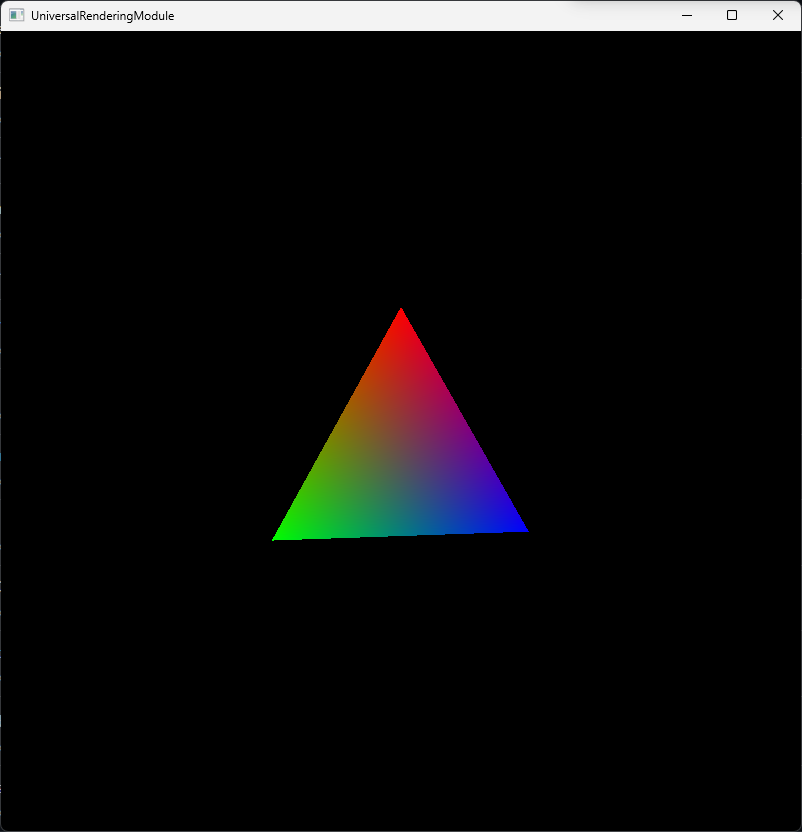
\includegraphics[width=300px]{images/impl/2_rotating_triangle.png}
	\caption{Rekreacja projektu zapoznawczego przy pomocy API modułu.}
	\label{Impl_RotatingTriangle}
\end{figure}

\section{Warstwa sceny}
Po ukończeniu warstwy rdzeniowej przyszła kolej na część sceny. Implementacja jej funkcjonalności rozpoczęła się od utworzenia bazowego obiektu sceny oraz struktury nimi zarządzającej - \textbf{Scene}. Następnie zaimplementowane zostały metody tworzenia, usuwania oraz przypisywania do hierarchii obiektów - odpowiednio \textit{Instantiate()}, \textit{Destroy()} i \textit{SetParent()}. Wzajemna hierarchia obiektów musiała zostać podparta strukturą zarządzającą ich wzajemnymi relacjami oraz transformacjami przestrzennymi, w związku z czym powstała odpowiedzialna za to klasa \textbf{Transform}, wykorzystująca macierze transformacji do odwzorowania wzajemnych relacji między obiektami.

\subsection{Gimbal Lock}
Jednym z częściej spotykanych problemów w reprezentacji transformacji jest rotacja. Jej intuicyjna implementacja w postaci wektora trzech elementów reprezentujących rotację w 3 osiach przestrzeni jest bowiem podatna na błąd zwany \textit{Gimbal Lock}. Jest to sytuacja, w której wraz z obrotem obiektu obraca się także układ współrzędnych wokół którego jest on obracany, a w rezultacie wykonanie tych samych rotacji w innej kolejności może doprowadzić do innej pozycji wynikowej, co zostało pokazane na rys. \ref{GimbalLock}.

Rozwiązaniem jest dodanie czwartego wymiaru o aktywnym balansie, określającego "niezależny" układ współrzędnych. Standardem realizacji tego konceptu jest struktura kwaternionów, która po dodaniu metod balansujących idealnie nadaje się do reprezentacji rotacji w przestrzeni trójwymiarowej. Do dalszej pracy użyta została implementacja \textit{Quaternion} zawarta w ramach pakietu SimpleMath.

\vfill

\begin{figure}[h!]
	\centering
	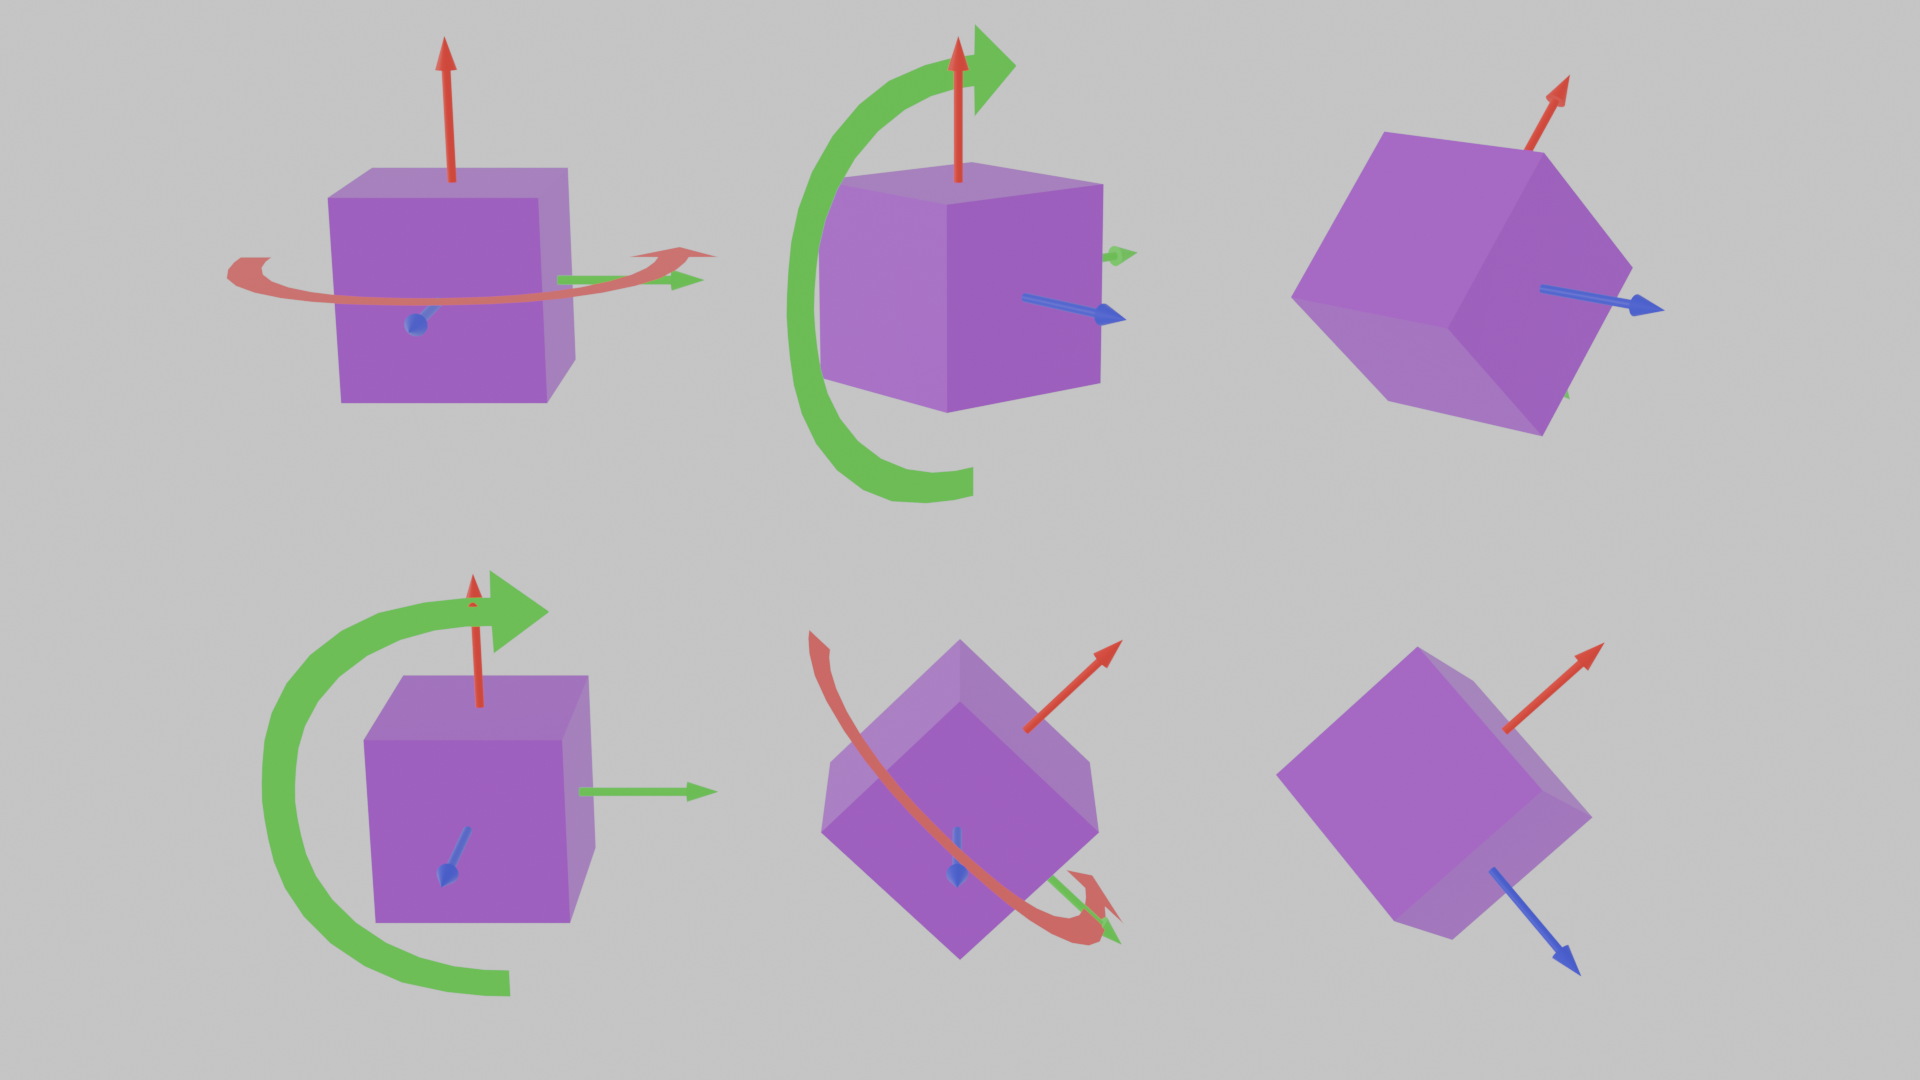
\includegraphics[width=\textwidth]{images/gimbal_lock.png}
	\caption{Wizualizacja efektu gimbal lock.}
	\label{GimbalLock}
\end{figure}

\subsection{Transformacje w przestrzeni}
Autor miał już doświadczenie w projektowaniu komponentów zbliżonych do \textit{Transform}, ale opierało się ono na API OpenGL i bibliotece GLM, zamiast użytego w projekcie Direct3D i DirectXTK / SimpleMath. Większość metod udało się utworzyć z małymi zmianami, ale problemem okazała się być metoda \textit{LookAt(target, upVector)}, która obraca obiekt w stronę przekazanej w ramach parametru \textit{target} docelowej pozycji w przestrzeni. Pakiet GLM zawiera dedykowaną do tego funkcja glm::lookAt() \cite{glm:docs:look_at}, której odpowiednika brakuje w pakiecie DirectXTK, więc funkcjonalność musiała zostać odtworzona. 

Pierwszym podejściem była próba wykorzystania dostępnej w DXTK metody \textit{XMMatrixLookAtLH()}, tworzącej macierz transformacji odpowiadającą rotacji kamery patrzącej na odpowiedni punkt. Wynikową strukturę należy następnie odwrócić, aby przekonwertować ją na wersję dla obiektu i na jej podstawie utworzyć kwaternion rotacji. 

\subsection{Problemy z wydajnością konstruktorów kopiujących}
W trakcie tworzenia modułu okazjonalnie sprawdzana była jego wydajność, która przez większość czasu wahała się w okolicach 10.000 FPS \textit{(ang. Frames Per Second)}. Była to przyjęta granica wynikająca z limitów innych niż wydajność samego modułu, gdyż minimalna aplikacja testowa składająca się jedynie z logiki czyszczenia i prezentowania klatek obrazu nie przekraczała tego poziomu wydajności. 

W okolicach tego punktu zauważony został jednak nagły spadek do poziomu około 2.000 FPS, mimo użycia sceny identycznej do pierwotnej - obracającego się trójkąta. Po analizie problemem okazało się przekazywanie wielu struktur, takich jak lista wierzchołków, w formie kopiującej zamiast referencji. Zmiana problematycznych wystąpień naprawiła problem, ale nie gwarantowała, że nie wróci on w przyszłości. Standard C++ od wersji 11 zawiera słowo kluczowe \textbf{auto}, które automatycznie określa typ zmiennej na podstawie przypisanej do niej wartości. Mechanizm ten nie obejmuje detekcji referencji i wskaźników, co spada na ręce programistów, nie pokazując przy tym żadnego błędu ani ostrzeżenia w przypadku użycia konstruktora kopiującego zamiast referencyjnego, a czego przykład został pokazany na listingu \ref{lst:module:cppcopyingref}. W związku z tym aby zapobiec przypadkowemu użyciu spowalniającej działanie programu metody kopiującej wprowadzona została pomocnicza klasa \textbf{NonCopyable}, która wyłącza konstruktory kopiujące w każdej klasie z niej dziedziczącej, pozostawiając przy tym dostępny mechanizm przenoszenia przy pomocy \textit{std::move}. W ten sposób oznaczone zostały najważniejsze klasy, takie jak \textit{D3DCore}, \textit{Window}, \textit{Scene}, a później także \textit{Engine}. 

\begin{lstlisting}[caption={Przykład sytuacji, w której łatwym jest użycie formy kopiującej zamiast referencji, co skutkuje dużym kosztem wydajnościowym.}, label={lst:module:cppcopyingref}]
	class Data {
		int field = 5;
	};
	
	class DataHolder {
		Data data;	
	public:
		Data& GetData() {
			return data;
		}
	};

	int main() {
		DataHolder holder;

		// Wywołanie konstruktora kopiującego
		auto data = holder.GetData();

		// Poprawna forma referencyjna
		auto& dataRef = holder.GetData();
	}	
\end{lstlisting}

\subsection{Podsumowanie modułu sceny}
Warstwa scenowa nie przyniosła wyraźnych zysków ani spadku wydajności, a także nie uprościła znacząco kodu klienckiego w przypadku testowego programu z trójkątem. Pozwoliła ona jednak na łatwą obsługę znacznie większych objętościowo światów, a także postawiła podwaliny pod kolejny submoduł - warstwę silnika.

\section{Moduł silnika}
Prace nad warstwą rozpoczęto od wydzielenia nowego projektu i utworzenia odpowiedniej klasy - \textbf{Engine}, mającej przejąć większość obowiązków związanych z rysowaniem modeli, zarządzaniem sceną i stanem związanym z obiektami niższych warstw zarządzającymi komunikacją z API Direct3D. Początkowo zaimplementowane funkcjonalności były jedynie przeniesieniem już istniejących funkcji z \textit{TestApp}, ale z czasem dzięki ustrukturyzowanej budowie modułu możliwe było dodanie nowych, bardziej złożonych funkcjonalności. 

\subsection{Niestandardowe programy cieniujące}
Pierwszą taką funkcjonalnością było dodanie obsługi niestandardowych shader'ów. Aby było to możliwe musiał jednak najpierw powstać ustalony schemat danych do nich oraz między nimi przesyłanych. W tym celu utworzone zostały współdzielone pliki kodu HLSL - \textbf{PixelShaderCommonTypes.hlsl} oraz \textbf{PixelShaderCommon.hlsl} - zawierających odpowiednio podstawową strukturę przesyłaną między Vertex i Pixel shader'ami oraz współdzielone struktury drugiego z nich, takie jak \textbf{Light} dla świateł i funkcja \textbf{CalculateLighting} obliczająca na ich podstawie prosty model oświetlenia. W późniejszej części dodane zostały w tym miejscu struktury opisujące dodatkowe parametry renderowanych obiektów, takie jak właściwości materiału czy oświetlenie typu PBR.

\subsection{Konflikt wydajność, a modularność}
Prawie każda decyzja projektowa poza oczywistymi zaletami ciągnie za sobą także wady. W przypadku tematu modularności częstym problemem jest ograniczony potencjał optymalizacyjny, ze względu na konieczność zachowania odpowiedniej struktury oraz brak możliwości wysokopoziomowej optymalizacji międzymodułowej. Autor zdawał sobie sprawę z tego kompromisu projektując opisywany system i stawiając przede wszystkim na modularność kosztem wydajności, ale w momencie integracji sceny z silnikiem doszło do bariery, która wymagała kompromisu na tym polu. 

Problemem okazało się przechowywanie obiektów typu cache w ramach struktury sceny, pozwalających na ograniczenie konieczności każdorazowego jej przechodzenia w celu znalezienia obiektów konkretnego, często używanego typu. Pierwszym takim przykładem była lista aktywnych w scenie modeli oraz świateł, która jest krytyczna do przyspieszenia procesu renderowania, gdyż każdorazowe przechodzenie sceny w ich poszukiwaniu przy każdym rozpoczęciu procesu rysowania wiązałoby się z dużym i stałym narzutem obliczeniowym. Problemem okazało się jednak gdzie taką listę umieścić. Intuicyjną myślą było dodanie takiego elementu do Sceny, ale nie było to możliwe, gdyż przez jej niezależność obiekt opisujący model lub światło w scenie z założenia nie mógł znajdować się w ramach tej samej warstwy, a dopiero na wyższym poziomie silnika. Takie ułożenie kłóciło się jednak z wcześniejszym założeniem, w którym niższa warstwa nie może odnosić się do obiektów z warstwy wyższej. Podobny problem byłby także gdyby umieścić listę w klasie \textit{Engine}, a dokładnie wymagałby on referencji do silnika w ramach struktury \textit{SceneObject}, będącej opisem obiektu sceny i znajdującej się na jej warstwie, co oznaczałoby konieczność odniesienia się do wyższego poziomu. 

Pierwszym testowym rozwiązaniem było dodanie do sceny wskaźnika pustego typu \textit{void*}, do którego przypisywana byłaby z wyższej warstwy struktura przechowująca potrzebne do działania dane. Problem pojawił się jednak w momencie zwalniania pamięci takiego obiektu, gdyż przez brak określonego typu nie było możliwe automatyczne wywoływanie destruktora takiej klasy, w efekcie czego pojawić się mogły wycieki pamięci. Rozwiązaniem byłoby dodanie kolejnego parametru w postaci wskaźnika funkcji destruktora, ale w połączeniu z już problematycznym interfejsem pobierania takiej struktury - brak gwarancji, że dane będą typu oczekiwanego przez warstwę klienta - podjęta została decyzja o odrzuceniu tej wersji naprawy problemu. 

Drugą wersją byłoby utworzenie interfejsu typu \textit{IScene}, z którego następnie tworzone byłyby implementacje zawierające potrzebne dane. Niestety takie podejście także cierpi na konieczność walidacji typu danych przez obiekty sceny i ich pobierania przy pomocy niebezpiecznych konwersji, w związku z czym ta opcja i jej podobne także zostały odrzucone. 

Ostatecznie przyjętym rozwiązaniem był kompromis na płaszczyźnie modularności. Warstwa rdzeniowa pozostała zupełnie niezależnym od pozostałych tworem, ale poziomy sceny i silnika zostały zintegrowane do jednej, wspólnej warstwy. Struktury cache umieszczono w ramach klasy \textit{Scene}. Takie podejście narzuca jednak problem z rozszerzalnością nowego, zunifikowanego modułu, gdyż nie ma bezpośredniej możliwości rozszerzenia jej o dodatkowe cache'owane dane. W związku z tym podjęta została decyzja o zmianie formy dystrybucji biblioteki na open-source. W większości docelowych przypadków użycia modułu nie będzie konieczności modyfikacji danych przechowywanych w ramach sceny i w takich przypadkach możliwe jest korzystanie z niego w formie prekompilowanej biblioteki, ale jeśli taka konieczność nastąpi to możliwe i zalecane jest dodanie warstwy silnika (z uwzględnioną w niej funkcjonalnością sceny) jako biblioteki w formie zintegrowanego do aplikacji klienta, modyfikowalnego kodu źródłowego. 

\subsection{DPI awareness}
Drobnym, ale istotnym problemem okazało się zachowanie aplikacji w przypadku konfiguracji komputerowych, w których skalowanie ekranu ustawione jest na wartość inną niż 100\%. System Windows raportuje w takich przypadkach rozdzielczość ekranu pomniejszoną o współczynnik skali, a następnie skaluje okna aplikacji o jej wartość. Dla przykładu przy skalowaniu 200\% i rozdzielczości monitora 4000x2000, system raportuje do aplikacji wartość 2000x1000, a następnie dwukrotnie skaluje jej okno, czego efektem jest rozmyty, niewyraźny obraz, co w wyolbrzymionej formie pokazane zostało na rys. \ref{Impl_DpiAwareness}.

Rozwiązaniem jest załączenie do modułu tzw. manifest'u, czyli informacji o obsługiwanych przez aplikację funkcjach i uwzględnienie wśród nich DPI Awareness. Aplikacja raportująca wsparcie tego rozszerzenia nie jest traktowana przez system w opisany sposób, a zamiast tego otrzymuje prawdziwe informacje o monitorze i nie jest ona skalowana. W przypadku aplikacji renderujących trójwymiarową grafikę jest to preferowany sposób działania i w związku z tym manifest został dodany do modułu. 

\begin{figure}[h!]
	\centering
	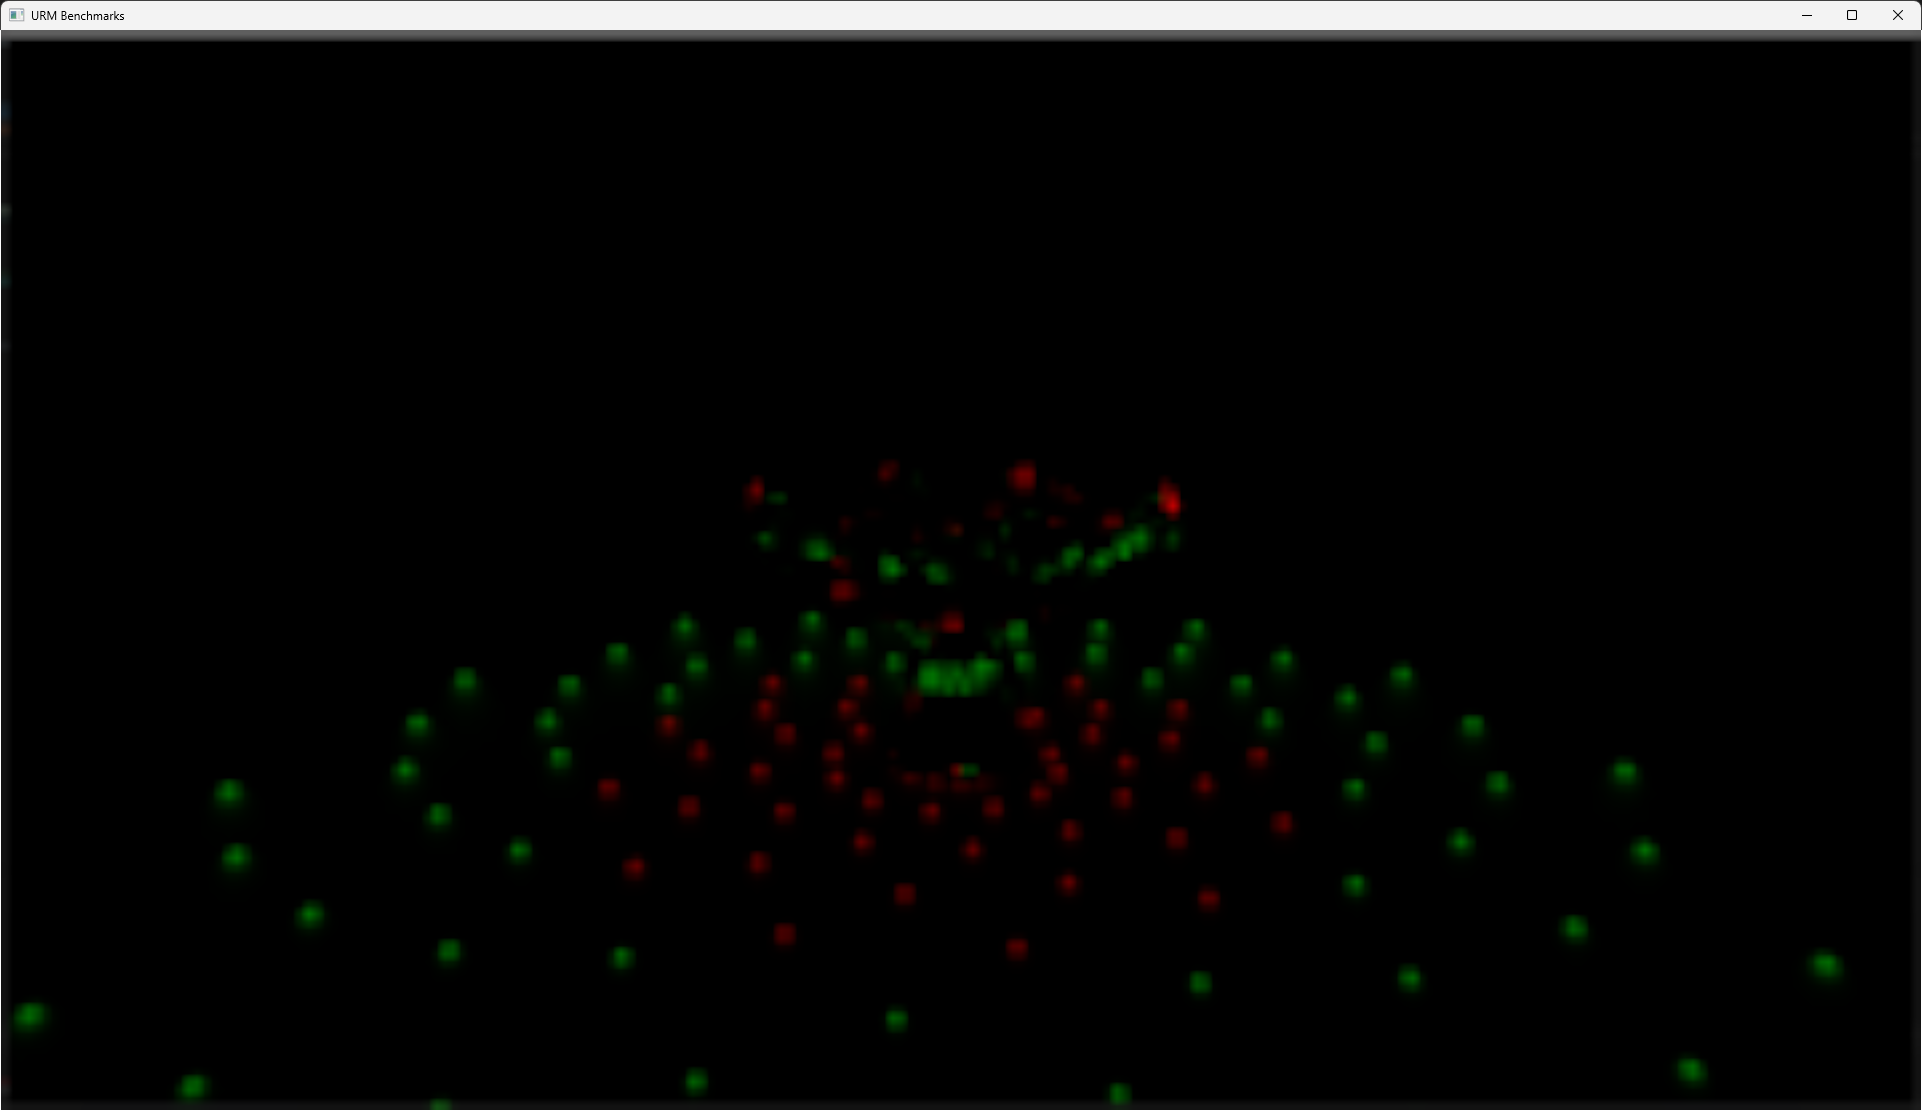
\includegraphics[width=\textwidth]{images/impl/4_dpi_awareness_8x.png}
	\caption{Wizualizacja efektu rozmycia przy braku DPI awareness aplikacji - na przykładzie dla skalowania 800\%.}
	\label{Impl_DpiAwareness}
\end{figure}

\vfill

\subsection{Caching wczytywanych modeli}
Dekodowanie danych o modelach oraz ich wczytywanie z dysku jest zadaniem wymagającym pod względem wymaganej mocy obliczeniowej i czasu potrzebnego do przetworzenia takich danych. Często spotykanym w świecie trójwymiarowych scen jest też zachowanie aplikacji, w których wczytują one pojedynczy model do wielokrotnego wykorzystania - na przykład krzak w grze z otwartym światem. Przy takim zachowaniu marnotrawnym byłoby każdorazowe przechodzenie przez proces wczytywania i dekodowania danych o tym samym modelu z dysku, więc w ramach modułu silnika utworzony został mechanizm zarządzania zasobami w postaci klasy \textbf{AssetManager}. Przechowuje ona wczytane modele i tekstury do późniejszego wykorzystania, ale pozwala także na ich zwolnienie przy zmianie sceny albo w sytuacjach o zmniejszonej dostępności wolnej pamięci podręcznej. 

\subsection{PBR i system materiałów}
Renderowanie oparte o PBR \textit{(ang. Physically Based Rendering)} jest aktualnym standardem w branży grafiki trójwymiarowej, więc obsługa renderowania o ten standard opartego została dodana do warstwy silnika. Z założenia modularności wynika jednak, że nie powinien być to jedyny wspierany system oświetlenia. Pierwszą próbą połączenia różnych typów kalkulacji świateł było wydzielenie najważniejszych komponentów Pixel Shader'a do osobnego pliku i dalszego wykorzystania. Chcąc utworzyć funkcjonalność jak najbardziej otwartą koniecznym było jednak zadbanie o nieograniczanie aplikacji klienta w kwestii tworzenia nowych, dowolnie skonstruowanych i rozwiniętych materiałów. W związku z tym wprowadzony został rozwinięty względem warstwy rdzeniowej system materiałów. Opiera się on na bazowej klasie \textbf{Material}, definiującej użyty do materiału Pixel Shader oraz przesyłanego do niego dane w postaci struktury typu \textbf{ConstantBuffer} i pozwala na zaimplementowanie wirtualnie dowolnej kombinacji materiału i programu cieniującego. 

Największym problemem związanym z takim systemem okazało się jego połączenie z autodetekcją materiałów wczytywanych modeli. Została tutaj podjęta decyzja o ograniczeniu wsparcia tego mechanizmu jedynie do oświetlenia typu PBR, ale pozostawienie możliwości ręcznej implementacji podobnej funkcjonalności na podstawie opisanych przy okazji warstwy rdzeniowej \textit{MaterialProperties}. 